\documentclass[]{article}
\usepackage{float}
%\usepackage{graphics}
\usepackage{graphicx}

%opening
\title{RAS Internal communication interface standards}
\author{Bart Boogmans}

\begin{document}

\maketitle
 
 \begin{figure}[H]
	\centering
	
\includegraphics{YW_RAS_logo_GreyBackground.png}
\end{figure}
 
\vfill
\begin{table}[H]
	\centering
	\begin{tabular}{lll}
		Date       & Name          & Description \\ \hline
		2022-08-29 & Bart Boogmans & Creation, initial layout, add namepace definitions  \\
		2022-09-6	& Bart Boogmans	& Add first coordinate systems \& messageformats      
	\end{tabular}
	\caption{Revision history of this document}
\end{table}

Note: This is an early file version. Interfaces described in this document are prone to change. 

\newpage
\section{Namespaces}
The following identifiers are used for our vessels:

\begin{table}[H]
	\centering
	\begin{tabular}{lll}
		Model    & Description          & Identifier  \\ \hline
		TitoNeri & Light-blue Tito Neri & RAS\_TN\_LB \\
		TitoNeri & Dark-blue Tito Neri        & RAS\_TN\_DB \\
		TitoNeri & Red Tito Neri        & RAS\_TN\_RE \\
		TitoNeri & Yellow Tito Neri        & RAS\_TN\_YE \\
		TitoNeri & Purple Tito Neri        & RAS\_TN\_PU \\

		TitoNeri & Green Tito Neri        & RAS\_TN\_GR \\
		TitoNeri & Orange Tito Neri        & RAS\_TN\_OR \\
		GreySeabax & The Grey-seabax        & RAS\_GS \\
		Delfia-1* & Delfia 1       & RAS\_DF\_1 \\
		Delfia-1* & Delfia 2       & RAS\_DF\_2 \\
		Delfia-1* & Delfia 3       & RAS\_DF\_3 \\
		Delfia-1* & Delfia 4       & RAS\_DF\_4 \\
		Delfia-1* & Delfia 5       & RAS\_DF\_5 
		
	\end{tabular}
\end{table}

\section{ROS topics \& message formats}

\begin{table}[H]
	\begin{tabular}{llll}
		Topicname & Description & Messagetype & Default unit(s) \\ \hline
		
		/\textless{}vesselID\textgreater{}/u\_ref & Actuator reference  & Float32MultiArray* & \begin{tabular}[c]{@{}l@{}}shaft velocities: Rpm\\ Azimuth angles: radians\\ pwm signal: normalized{[}-1:1{]}\end{tabular} \\
		
		/\textless{}vesselID\textgreater{}/u\_est & Measured actuator state & Float32MultiArray & identical to /\textless{}vesselID\textgreater{}/u\_ref \\
		
		OptiRAS/\textless{}vesselID\textgreater{} & Estimated pose & stdmsgs/pose & meters,quaternions \\
		
		/\textless{}vesselID\textgreater{}/x\_est & Estimated surface state & type & unit \\
		name & desc & type & unit \\
		name & desc & type & unit 
	\end{tabular}
\end{table}

* for the delfia this refers to $[rps\_back,rps\_front,angle\_back,angle\_front]$\\
for the TitoNeri this refers to $u = [rpm\_PS\_thr,rpm\_SB\_thr,pwm\_bow,alpha\_PS\_azi,alpha\_SB\_azi]$\\

- standard variations: (e.g. pose as 3 or 6 DOF.) and how to distinct them, and when we generally use which one. 

\section{IP reservation}
explain local network and vpn server protocols.
explain how to connect to both. 


\section{Coordinate systems}
\subsection{Tiny lab tank}
The coordinate system of the optitrack system on the tiny lab tank is defined as follows:

\begin{figure}[H]
	\centering
	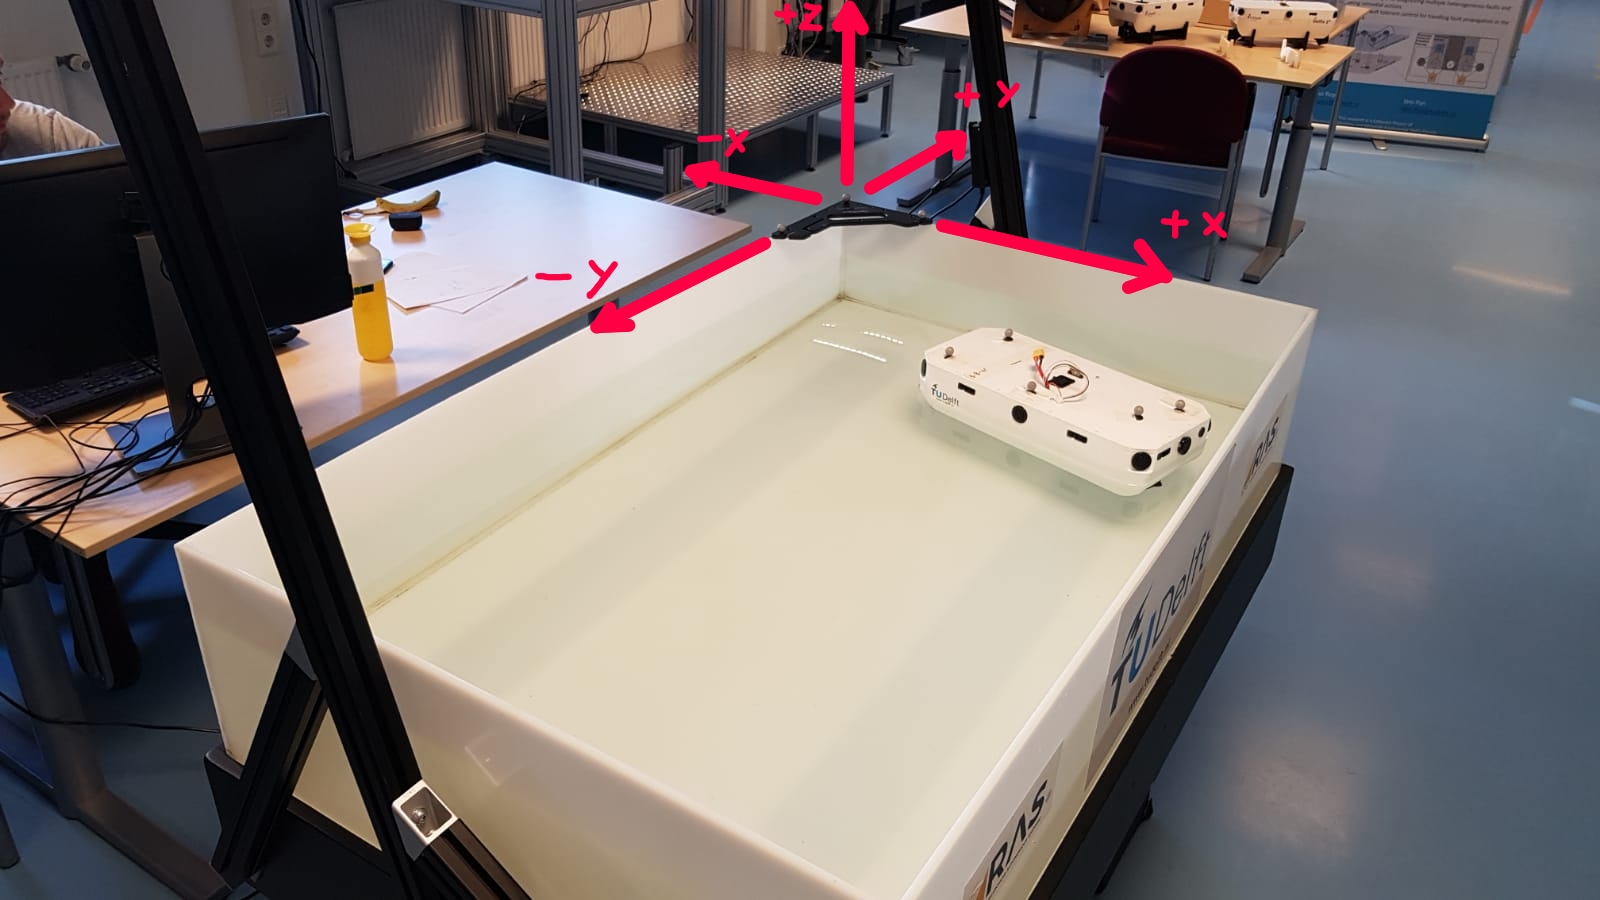
\includegraphics[width=0.8\paperwidth]{tinyTank1_labeled.jpg}
	\caption{The tiny tank is about 1.3 by 0.81m}
\end{figure}
Note that Z does not point down (as in line with the standard NED definition). Coordinate system transformation can be done afterwards, but this is how you can expect the initial pose-stream on ROS.

\subsection{Small towing tank}
TBD

\end{document}
